% !TeX spellcheck = da_DK
\documentclass[11pt, fleqn]{article}
%\usepackage{siunitx}
\usepackage{texfiles/SpeedyGonzales}
\usepackage{texfiles/MediocreMike}
\title{02466 Project work in Artificial Intelligence and Data LOGBOOK}
\author{Oskar Eiler Wiese Christensen s183917, Anders Henriksen s183904, Dagh}

\begin{document}
	\maketitle
		
\section*{Project Meetings}
	
	%Questions \\
	%Reading, who and what \\
	%Implementation, who and what \\
	%Results, who and what \\
	%Decisions, who and what, what do you do alone, what do you do together
	
	\textbf{Week 08:}  19.02.2020 \\\\
	\noindent
	Hvilke bias eksisterer i dataen? \\ 
	\begin{figure}[H]
		\centering
		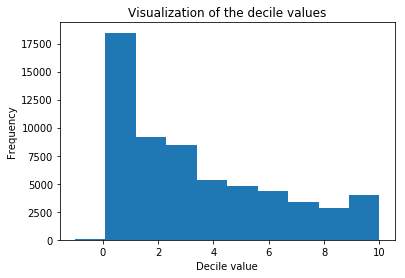
\includegraphics[width=0.3\linewidth]{billeder/decil.png}
	\end{figure}

	\begin{figure}[H]
		\centering
		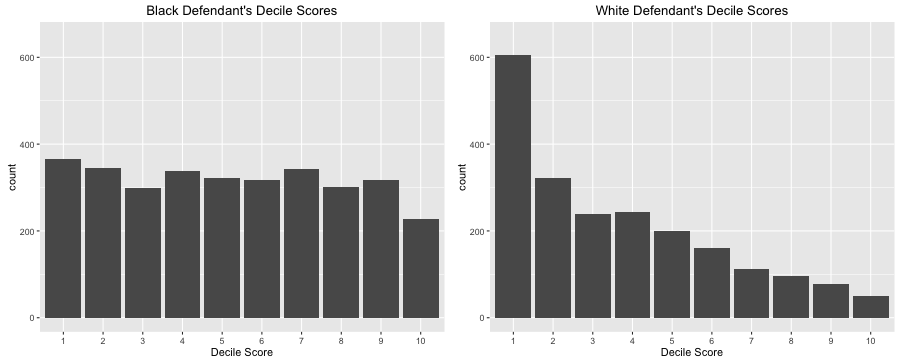
\includegraphics[width=0.7\linewidth]{billeder/black_white}
	\end{figure}
	\noindent
	There exists a recial bias in the dataset, which is indicated by the histograms above. 
	\\\\
	\textbf{Week 10:}  03.03.2020 \\\\
	\noindent
	Spørgsmål til næste møde: \\
	Hvordan skal dataen permuteres ? (Kun indenfor en kategorisk variabel eller hele datasættet) \newline 
	Kan man se bias ud fra confusion matrix?? \\ 
	Skal man vise, at der en statistisk forskel på de to confusion matricer? \\ \\
	\textbf{Noter} \\ 
	Lav nogle flere plots for at vise, om der er bias i selve data. Undersøg, hvor mange der får 1 i recidivism både af sorte og hvide.
	\newline
	Det ville være smart at finde noget statistisk signifikans. Man kan finde en p-værdi ved at bruge permutationstests.
	\newline
	Lav predictions med random forests.
	\newline
	Equal opportunity er godt resultatet, som vi ser fra vores data. Man kunne plotte equal opportunity som netværket bliver trænet.
	\newline
	Lav en slags baseline som logistisk regression for at se, om de begge er biased eller om de klarer sig lige godt.
	\newline
	Vi skal senest have midvejafleveringen klar d. 16, så Aasa kan læse det igennem.	
	\\\\	
	\textbf{Week 11:}  10.03.2020 \\\\
	\noindent
	Spørgsmål:
	\begin{itemize}
		\item  Hvordan skal vi lave feature selection for at se om de forskellige attributes påvirker modellen? Skal det stå som et afsnit i metoder?
		
		\item 4454, i forhold til at tage udgangspunkt i dataen, hvordan kan bias påvises vha. permutationstest. 
		
		\item Hvordan man helt præcist skal implementere Hardt et al. (post hoc correction)
		
	\end{itemize}
	
	
	
\section*{Supervisor Meetings}
	
	\textbf{Week 07:}  12.02.2020 \\\\
	\noindent
%	Presentation of results since last meeting \\
	Meeting notes: \\ Fællesmøder samt personlige møde. (Hver anden uge er individuele). \\0. Vi får et datasæt (COMPASS) - ligger online \\
	1. Hvordan er dataen skæv? (Hvilke bias eksisterer i dataen) (Hvordan finder man helt præcist ud af det?) (Hvad betyder det at der er en bias?) \\
	2. Hvad gør skæv data ved min algoritme? (hvad betyder bias i en algoritme) (Hvordan kvantificeres/verificeres bias i algorimten?) \\
	3. Equality of Opportunity in Supervised Learning (forstå, implementer og valider) \\ 
	4. Etisk diskussion (Sune Filosof)
	\\\\\\\\
	\textbf{Week 08:}  19.02.2020 \\\\
	\noindent
	%	Presentation of results since last meeting \\
	Meeting notes: \\ Feature extraction
	\\\\
	Action points for next week: N/A
	\\\\\\\\
	\textbf{Week 09:}  26.02.2020 \\\\
	\noindent
	%	Presentation of results since last meeting \\
	Meeting notes: 
	\\\\
	Action points for next week
	\begin{itemize}
		\item  
	\end{itemize}

\section*{Definition af Bias:}
	
	Bias i datasæt 
		
	
\end{document}
